\chapter{Work Done}

This section details the development work that has been performed in the second phrase of the project.  This includes conceptual problems faced, effectiveness of the result and any future work that could be performed.

%For each of the below, why, how inc conceptual problems, impact, how it could be improved


\section{Animation}

THIS NEEDS A LOT OF WORK

Animation was a key goal of the project.  The core aim of the project is to help biologists who aren't comfortable with traditional time-series graphs.  So the goal was to provide them with visualisations closer to what they see in their domain.  This has been accomplished by displaying spatial data in the shape of the cell.

The animation is ideally used to display species moving through a cell.  This collapses what would be multiple different lines in a graph, that give no indication of their real position in the cell, into a single image.  There is one segment in the cell animation for each line.  The colours in each segment reflect the colour of the line on the graph.  Then over the course of the animation the colours are set by the colour in the intensity plot version of the line.  This allows the researcher to compare the two visualisations and will hopefully help build their confidence on the graph plot.

To make setting up the animation user friendly to control required the model file so that the location hierarchy could be parsed.  Before this there was an awkward system where the user had to input where in the cell a species is.  This was time consuming, awkward and quite brittle.  At the time it assumed that there would be three compartments in the species, which is a terrible assumption to make.

The requirement of the model file for parsing animation has also led to animation replacing the previous model visualisation.  In the set up phase after the the model and the species have been parsed the user is presented with a cell segment, similar to what is seen in the animation panel.  The cell segment is split into different regions, one for each region of the cell.  These segments are then coloured if the selected species is present in them.  The user can select between all species in the selected results files.  This has a number of benefits.  First, they can sanity check that they have matching results and model files.  Second, they can see how the model is structured.

Similar control is provided on the animation panel itself.  The user can see the animation focused on a specific species, in which case a cell segment is drawn for each file that the species is in.  Or they can have the animation focused on a specific results file in which case a cell segment is drawn for each species in that results file.

\section{Annotation}

Annotation was an important feature to add.  It is one of Grinstein's features that data visualisation software should have~\cite{gg_vizbi}.  This is because the purpose of a visualisation is to aid analysis.  If you have a print out of a visualisation you are able draw on it and highlight areas of interest.  Users need to be able to do this on digital versions of their visualisations.  As well as helping users analyse their data, being able to annotate also means that images for presentations can be prepared without having to save the visualisation and open it in an external program.  If you did this and then wanted to change the visualisation you would have to re-annotate it.  This is frustrating for a user and wastes their time.  Being able to do it from within the visualisation solves this problem as the raw data and the annotation data are together.  Another benefit of being able to annotate is having another way of attaching additional information to the visualisation when sending it to a colleague. Having this information on the visualisation saves them from flicking back and forth from an email or other supporting documentation.

Implementing annotation of the visualisations on offer in this tool had to be done in two parts.  This is because there are two parts to the annotation.  The graph and the cell level view.  One is a static visualisation and one is a dynamic visualisation.  Each of these required a different approach.  These are detailed below.

\subsection{Annotation of the Graph}

Annotation on the graph was relatively straightforward to implement.  matplotlib provides annotation capabilities in two forms.  One form is annotations that use arrows with or without text, and the other is arbitrary drawing on the graph.  Both of these forms have been utilised for annotations.

Users of the new tool are provided with four annotation types: arrow, text, arrow with text and circles.  Buttons for each of these annotation types have been placed on the matplotlib toolbar.  This can be seen in Figure~\ref{fig:annotation_demo}

\begin{figure}[h!]
    \centering
    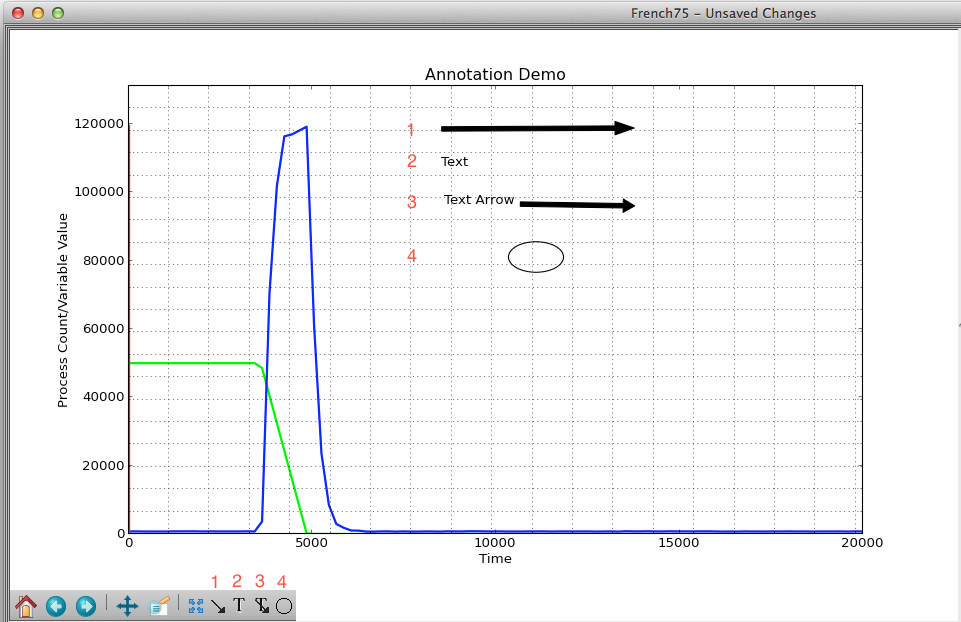
\includegraphics[width=\textwidth]{images/annotation_demo.png}
    \caption{Example of Each of the Four Annotation Types and the Toolbar Buttons that Correspond to Them}
    \label{fig:annotation_demo}
\end{figure}

There were problems in making the annotation creation process user friendly.  For all of the annotations the user needs to first press the appropriate button on the on the toolbar.  The next actions depend on the annotation type.  Text and circle annotations were intuitive as all they require is one click.  The user clicks where they want the annotation to be placed and it will be drawn on the graph there.  However the two arrow annotation types required two clicks.  The first click marks the start point (the tail of the arrow) and the second click is the finish point (the head of the arrow).  This was not obvious, when handed over to the users they didn't know that it required two clicks and didn't know whether the arrows would be drawn head to tail or tail to head.  The technique for placing arrows was changed so that the first click still fixed the position of the tail of the arrow. However the behaviour after the first click has changed, now a temporary annotation is continuously redrawn that has the head of the arrow wherever the mouse is.  This allows the user to see the arrow they are drawing.  To indicate to the user that they need to click on the graph the cursor is changed after pressing one of the annotation buttons on the toolbar.  The use of different cursors is a common technique to help guide users to perform actions.

It was important that annotations could be edited or deleted.  The annotations can not just be clicked as they are not a \ac{UI} widget like a button.  The solution to this was to have an array of annotations.  When a user right clicks on the graph it searches through all annotations and selects the annotation that was closest to the click (if that distance was below a certain threshold).  The selected annotation is then highlighted red, and a context menu appears to give feedback to the user that they have successfully selected an annotation.  This can be seen in Figure~\ref{fig:annotation_selection}  The context menu then gives the user the option to edit or delete an annotation.  Editing an annotation only allows for editing text.  For changing position the annotation has to be deleted and redrawn.

\begin{figure}[h!]
    \centering
    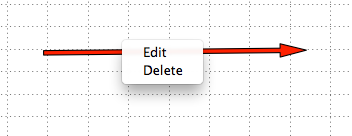
\includegraphics[width=\textwidth]{images/annotation_selection.png}
    \caption{Context Menu on Selection of Annotation}
    \label{fig:annotation_selection}
\end{figure}

To calculate the distance from the location of the mouse click to the annotation two problems had to be solved.  The first was how to calculate the distance from a point to a line.  An equation for this can be seen in Figure~\ref{fig:point_to_line_eq}.  Equation~\ref{eq:line} is the equation for a line in two dimensions.  This represents the annotation.  The equation can be calculated from the start and end points of the annotation. Equation~\ref{eq:point} is the position of the mouse click.  Equation~\ref{eq:distance} shows the equation for calculating the distance from the point to the line.  The second problem that had to be overcome was the difference in scale.  In effect we have two coordinate systems.  The results coordinate system and the visual coordinate system.  These difference are illustrated in Figure~\ref{fig:distance_scale}.  The annotations in Figure~\ref{fig:distance_scale_a} are further away from each other in the results coordinate system than the annotations in Figure~\ref{fig:distance_scale_b}, however they are closer in the visual coordinate system.  When selecting an annotation the user is using the visual coordinate system but the distance is calculated using the result coordinate space.  This could lead to the wrong annotation being selected.  The solution to this was to transfer one coordinate system into the other.  When calculating the distance from the point to the line the values are scaled by the size of the graph.

\begin{figure}[h!]
    \centering

    \begin{subfigure}[b]{\textwidth}
        \centering
        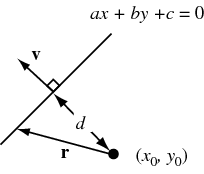
\includegraphics[width=0.3\textwidth]{images/point_to_line.png}
        \caption{Diagram of the Point to Line Distance Problem}
        \label{fig:point_to_line_diagram}
    \end{subfigure}

    \begin{subfigure}[b]{\textwidth}
        \begin{subequations}
            \begin{align}
            & y = -\frac{a}{b}x - \frac{c}{b} \label{eq:line}\\
            & (x_{0}, y_{0}) \label{eq:point} \\
            & d = \frac{\mid ax_{0} + by_{0} + c \mid}{\sqrt{a^{2} + b^{2}}} \label{eq:distance}
            \end{align}
        \end{subequations}
        \caption{Equations for Calculating the Distance From a Point to a Line.}
        \label{fig:point_to_line_equations}
    \end{subfigure}
    \caption{Equations and Diagram for Calculating the Distance From a Point to a Line (taken from WolframMathWorld~\cite{point_to_line})}
    \label{fig:point_to_line_eq}
\end{figure}

\begin{figure}[h!]
    \centering
    \begin{subfigure}[b]{0.6\textwidth}
        \centering
        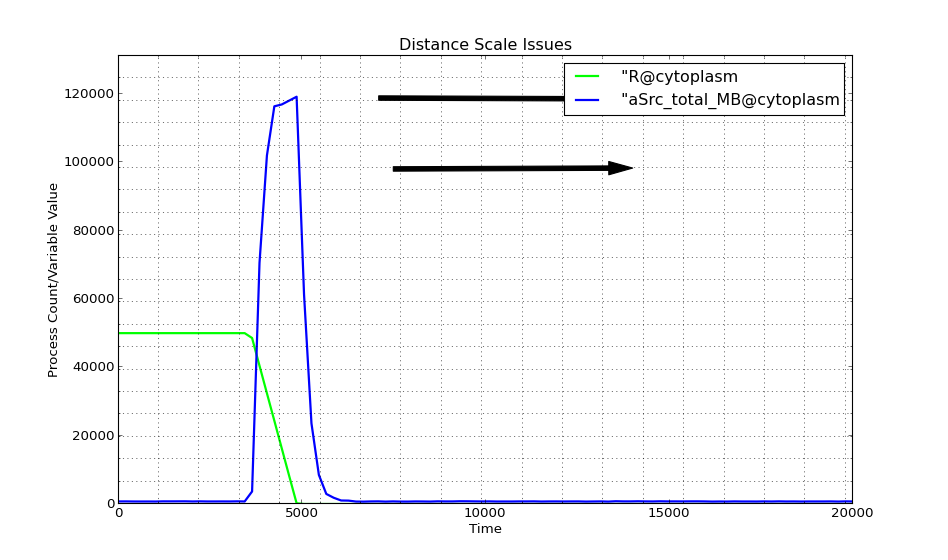
\includegraphics[width=\textwidth]{images/distance_scale_a.png}
        \caption{Annotations With Distance of Approximately 20000}
        \label{fig:distance_scale_a}
    \end{subfigure}

    \begin{subfigure}[b]{0.6\textwidth}
        \centering
        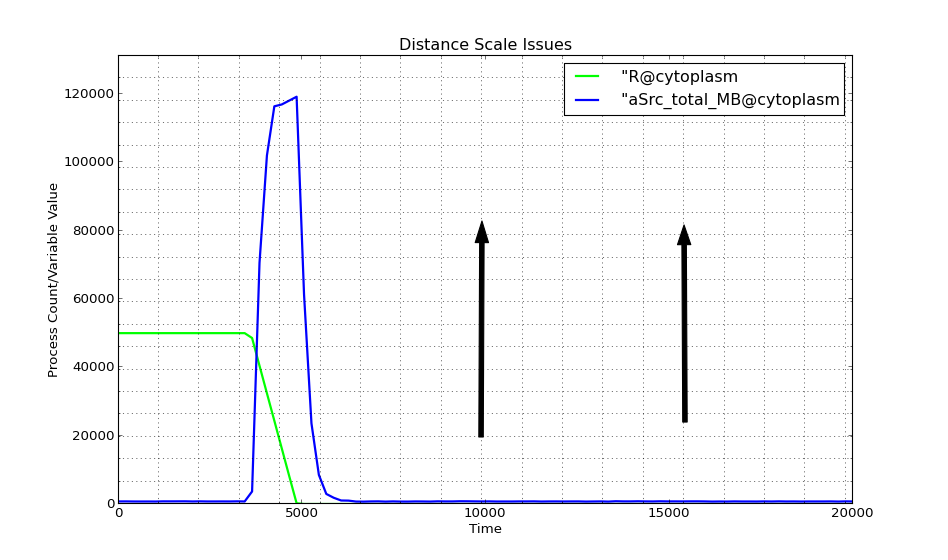
\includegraphics[width=\textwidth]{images/distance_scale_b.png}
        \caption{Annotations With Distance of Approximately 5000}
        \label{fig:distance_scale_b}
    \end{subfigure}
    \caption{Two Sets of Annotations Illustrating the Problems When Calculating Distance to an Annotation}
    \label{fig:distance_scale}
\end{figure}

A similar issue to the difference in scale when calculating the distance from the mouse to annotation was encountered when switching the graph to normalised mode.  When normalised the graph in the y axis only goes between 0 and 1.  The coordinates of the annotation are likely to be very much outside this range and the annotation would not appear on the graph.  The solution was to if the graph is normalised then to also normalise the positions of the annotations when drawing them.  A side effect of this technique is that the lines are potentially going to rescale themselves.  This could leave an annotation point to nothing.  This is unavoidable as the annotation has no concept of what it is pointing at.  It may be pointing to the intersection of more than one line, in this case it would be impossible to keep the annotation pointing at what it was originally pointing at.  Neither of these is optimal.  Both approaches lose the information that the user originally added.  During user evaluations, when the annotation would not be visible during data normalisation, the user was very confused as to why their annotation had disappeared.  It was therefore decided to have the annotation be visible but most likely incorrect as it is clearer to the user what has happened.

\begin{figure}[h!]
    \centering
    \begin{subfigure}[b]{0.6\textwidth}
        \centering
        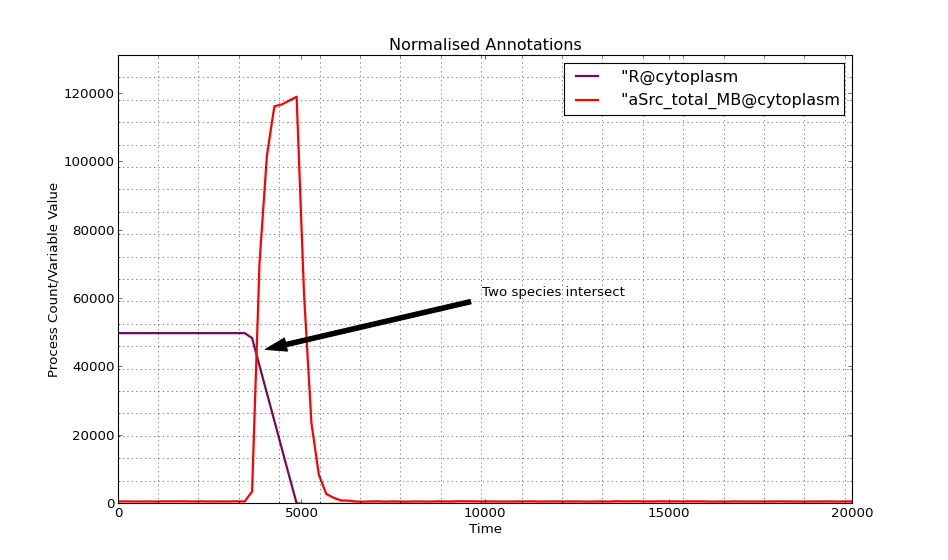
\includegraphics[width=\textwidth]{images/unnormalised_annotation.png}
        \caption{Annotation Pointing at Correct Intersection of Species}
        \label{fig:distance_scale_a}
    \end{subfigure}

    \begin{subfigure}[b]{0.6\textwidth}
        \centering
        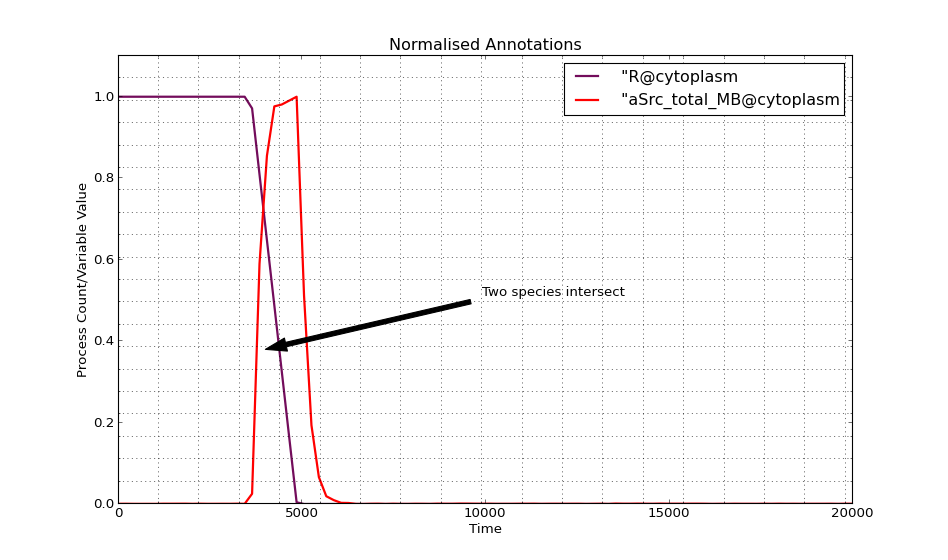
\includegraphics[width=\textwidth]{images/normalised_annotation.png}
        \caption{Annotation Pointing at Nothing After Data Normalisation}
        \label{fig:distance_scale_b}
    \end{subfigure}
    \caption{Graphs Illustrating What Happens to Annotations Whilst Data is Normalised}
    \label{fig:distance_scale}
\end{figure}

\subsection{Annotation of the Animation}

After completing annotation of the graph it was important to expand this to the animation panel, as this is the other visualisation option available to a user.  Annotating animations posed more of a challenge than annotation of the graph and there were a number of issues to overcome.

\begin{enumerate}
\item How to implement the annotations?  For the graph matplotlib has built in annotation support.  wxPython does have drawing support but not in built annotation support.  Annotating on the animation will need manual handling of the drawing on top of the animation visualisation.  Manual drawing means that the automatic layout functionality that wxPython provides cannot be used.
\item When to display the annotations?  When an annotation is drawn on the graph it is displayed at all times.  The appearance of the graph does not change over time.  However the appearance of the animation visualisation does change over time.  The problem faced when annotating is whether to have annotations available at only specific times in the animation, or to have them there the whole time, and if they are going to appear and disappear how can it be done without being distracting?
\item How to give the user control over the annotations? When a user wants to edit or delete an annotation on the graph it is always there.  However on the animation panel if the annotation is temporal, then it is not always visible for the user to edit or delete and it would be frustrating for a user to constantly have to search through the animation to look for annotations to change them.
\end{enumerate}

A platform where users are able to annotate an `animation' is YouTube~\cite{youtube}.  YouTube's annotation interface can be seen in Figure~\ref{fig:youtube}.  Youtube's approach is to allow the user to set what period of time an annotation is visible for.  There is also a management panel where the user can see all of the annotations and edit or delete them.  This approach solved issues two and three and was adapted for this tool.

\begin{figure}[h!]
    \centering
    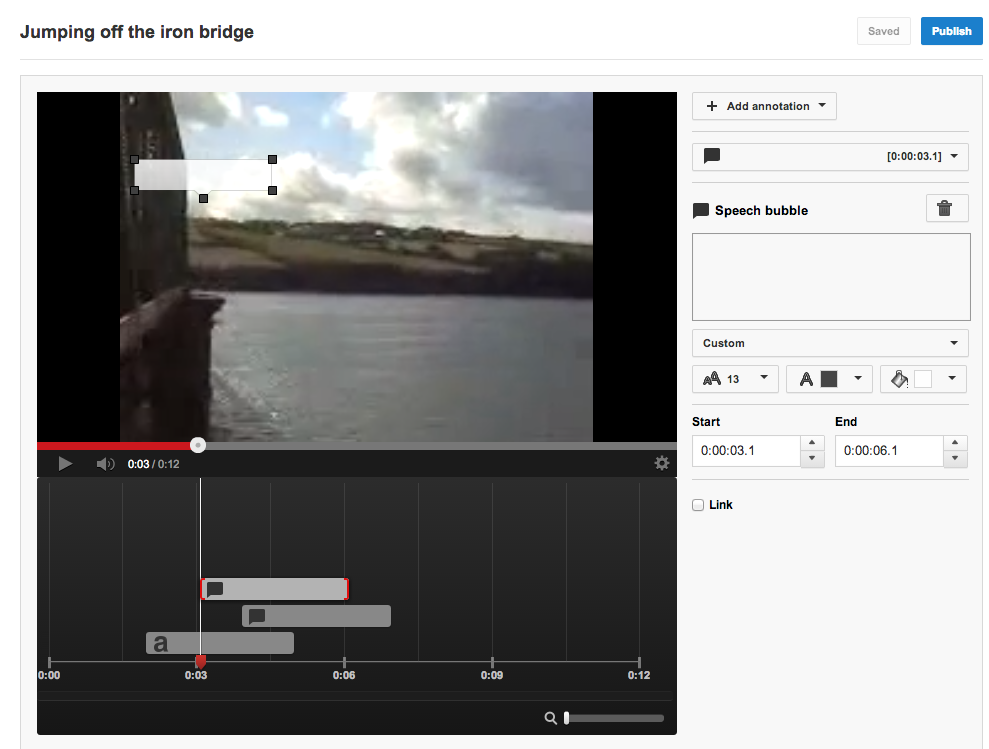
\includegraphics[width=0.7\textwidth]{images/youtube.png}
    \caption{YouTube Video Annotation Interface}
    \label{fig:youtube}
\end{figure}

On the right hand side of the tool there is a panel which lists all annotations that have currently been added to the tool, this can be seen in Figure~\ref{fig:annotatlion_list}.  This provides the user with the persistent view of what has been added.  When the user creates an annotation they are shown a dialogue that allows them to enter the annotation text and to choose a duration.  This indicates to the user that the annotation will only be visible at certain times.  The start and end times are given in model time.  The duration displayed to the user is given as the real time that the annotation will be visible for.  This can be seen in Figure~\ref{fig:annotation_dialog}.

\begin{figure}[h!]
    \centering
    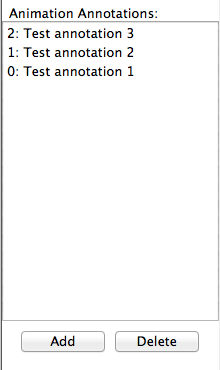
\includegraphics[width=0.7\textwidth]{images/annotation_list.png}
    \caption{Animation Annotation List}
    \label{fig:annotation_list}
\end{figure}

\begin{figure}[h!]
    \centering
    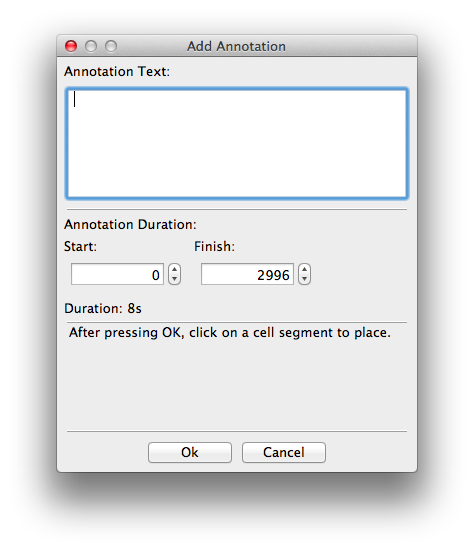
\includegraphics[width=0.7\textwidth]{images/annotation_dialog.png}
    \caption{Animation Annotation Dialogue}
    \label{fig:annotation_dialog}
\end{figure}

The first problem -- how to display the annotations -- has also been solved.  Drawing in wxPython takes place on panels.  Each cell cross section is placed on its own panel.  This drastically limits the available space.  The panels are not wide enough to have the annotation text drawn on.  The solution was to assign each annotation a number and that number is what is used to annotate the cell.  The number is then displayed in the annotation list box allowing the user to read the appropriate annotation.  This can be seen in Figure~\ref{fig:annotation_whole}

\begin{figure}[h!]
    \centering
    \begin{subfigure}[b]{0.4\textwidth}
        \centering
        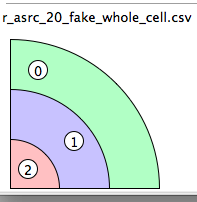
\includegraphics[width=0.9\textwidth]{images/annotation_whole_b.png}
        \caption{Annotated Cell Section}
        \label{fig:annotation_whole_cell}
    \end{subfigure}
    \begin{subfigure}[b]{0.4\textwidth}
        \centering
        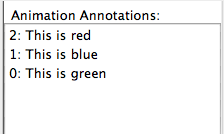
\includegraphics[width=0.9\textwidth]{images/annotation_whole_a.png}
        \caption{Corresponding Annotation List}
        \label{fig:annotation_whole_list}
    \end{subfigure}
    \caption{Animation Annotations}
    \label{fig:annotation_whole}
\end{figure}

\section{Data Mining}

\section{Search}

Using a time series as a plot posed some interesting problems.
\begin{itemize}
\item How to cope with different scales
\item How to cope with events happening at different times
\item How to represent the plot to allow for efficient search
\item How to determine similarity between two graphs
\end{itemize}

All of these needed to be overcome for this feature to be useful.

This is an area of active research.  Early techniques used simple techniques such as Euclidean distance, but these simple approaches gave poor results.  It is feasible to have a species that exhibits a similar reaction to our query (the line has the same shape) but it happens at a different time in the experiment than our query plot.  In other words the graph is offset.  We can tell that the two graphs are similar, but euclidean distance will return that they are unsimilar.  The same problem occurs with differences in species population giving an offset in the x axis.

After researching current techniques an approach was taken that solves all the problems above.

The first step is to convert the input data to be a list of all n length sub lists of the input data. i.e. with input data [1,2,3,4,5] and n = 3 our input data would become [[1,2,3], [2,3,4], [3,4,5]].  The sub lists are our features.  We then normalise each feature to be zero mean, unit variance.

The next step is to convert the continuous data into discrete data and reduce the dimensionality of it.  By normalising the data to be zero mean and unit variance we have allowed a normal distribution to be easily fitted to our data.   Using the normal distribution we convert a data point in our sub list to be one of three possible values.  Here we use the characters `a', `b' \& `c'.  This builds a string representation of the plot.

The paper this approach is taken from then calls for reducing local duplicates.  This further reduces the size of our fingerprint and increases the efficiency.  Removing the local duplicates means any ignoring runs of a certain string can be replaced with just one instance of the string.

This provides us with a finger print of the plot.  A string size of 8, with 3 possible value leads to a vocabulary size of 6561 possible representations.  A single plot will have very few of these, so we use a sparse representation.  For each line a dictionary is stored.  The dictionary keys are the strings in the fingerprints and the value is the count of that string in the plot's fingerprint.

This format of the fingerprint also solves the problem of similar features happening at different times.  The plot fingerprint is a bag-of-words, in this case a bag-of-features.  There is no order to them, it is as though we are assuming that all features appear at the same instant.

Now that we have a representation of the plot that is scale and time invariant and allows for efficient comparisons we can find a method to calculate the similarity.

We could simply just use Euclidean distance again, but this does not do anything to weight rarer features that can tell us more about a graph.  An alternative distance measure would be cosine distance, but this suffers the same drawback.

It was decided to implement tf.idf weighted cosine as the similarity measure.  This takes into account term frequencies to provide a higher weight to rarer vectors.  tf.idf is very well researched in the field of information retrieval and text mining.  Given the representation of the finger print is equivalent to a bag-of-words it seems sensible to apply tf.idf to this domain.

\subsection{tf.idf} is a way of ranking how important a word is.  Taken into account are frequency of a word in the query, frequency of a word in the document, length of the document, average length of documents in the corpus, total number of documents and frequency of the word across all documents.

The formula is: INSERT FORMULA.

These term weights are then used in a tf.idf weighted cosine.

This approach allows for effiecient search.  If we have two indexes.  One where keys are the documents and the values are the words in the document and their frequencies. Then we have another index, an inverted one.  Where the keys are the words and the values are a list of documents that contain them.  The individual components of the tf.idf equation can therefore be calculated with very little effort.  This means that a plot can be compared to the database of plots in O(n) time.

Initial results are very promising with the tf.idf weighted cosine providing much clearer results than with simple euclidean distance.  There is not a large enough truth set of plot similarities to be able to confidently say that it is effective.  However these early promising results seem to indicate that further research would certainly be worthwhile, but outside the scope of the project.

DISCUSSION OF THE EARLY RESULTS

\section{Collaboration}

The initial step of allowing collaboration is enabling two instances of the program to talk to each other.  There are a number of techniques to allow for this.  Data could have been sent directly through sockets, another option would be to create a web server and send get requests and pass parameters.  It was decided to use an existing library to handle the communication.  The library chose was simplexmlrpc.  This allows each instance to run a client and a server.  The server has an api and this can be called.

On initial connection the `master' sends its entire session state the the `slave' uses this as its initial state.  After this whenever either client performs an action it issues a call to the other clients server to perform the same action.

An issue that was encountered is how to ensure that both clients are seeing everything in the same order.  Lamport clock proved to be the solution.

\section{Usability}

In all the evaluations of the project users have commented on the difficulty of using parts of the tool.  Action has been taken to make it easier to use.  Many of the changes have been guided by Shneiderman, Norman \& Nielson's guidelines.  Specifics are detailed below.

\subsection{Undo \& Redo}
Shneiderman calls for easy reversal of actions and Nielson calls for user control and freedom -- an emergency exit from an unwanted state.  To address this, an undo/redo functionality has been added.  This required refactoring of the project code, so that the session data is in one location, inside a singleton. Any changes to this data are picked up during the next \ac{UI} update and are reflected in the visualisations.  The session data is stored as a dictionary.  To implement undo and redo, copies of the data dictionary are pushed and popped onto the stack.  Copies are pushed onto the undo stack on any atomic change the user makes.  This gives the user a full session history to go back through and this was one of the early goals from the first project phase.

A problem was encountered when trying to copy the dictionary onto the stack.  When just pushing the dictionary onto the stack it would not put a new copy of it onto the stack, so any changes to the dictionary after it has pushed onto the stack are also there in the stack.  Python dictionaries have a copy method.  Copy only does a shallow copy -- any objects in the original dictionary will have their reference placed in the new dictionary.  This was fine for some parts of the session dictionary, but for others it was not. In particular, lines and annotations, which are custom objects presented problems.  This was solved by using deep copy.  With deep copy a new copy is made of objects as well.  Some elements of wxPython and matplotlib were unable to be deep copied, but this was fixed whilst focusing more around the data -- so the \ac{UI} elements use the data, not the other way around.

\subsection{Saving}

It is important that a user is able to save and load the visualisation session as they may not be able to complete all their analysis in one sitting and may want to come back to their work in the future.  Without the ability to save and load the user would have to repeatedly add annotations and change preferences and attach files.  It was possible to add Saving and loadingby building on the work done to implement undo \& redo, although further work was required. Python has a module called pickle to serialise and deserialise data.  When saving, the dictionary containing the session data is pickled and written to a file and when loading the reverse happens.  Because the program is now focused on the data model, once a previous session has been loaded, a \ac{UI} refresh is triggered and the visualisation reflects the loaded data.

Saving the data also enables limited collaboration.  The user can customize the appearance and add annotations.  They can then save the state to a file and email that file to a colleague.  The colleague can then load the file and see the user's work.  The colleague can then correct any issues and add their own work.  The colleague can then save this and email it back to the user.  This is useful and is better than no collaboration, but it is entirely non realtime.

\subsection{Feedback}
Norman and Shneiderman both call for feedback to be given to the user so that the user can be sure that an action has been accomplished.  This feedback can come in a number of different forms and was in place in some parts of the project already.

Existing feedback in the project was a natural byproduct of some of the features; for example, when loading a results file the feedback that the load operation has been successful is that a graph appears on the screen. If the graph does not appear then something has gone wrong.  Additional feedback has been added to the project:
\begin{itemize}
\item When adding annotations the cursor changes to indicate to the user that they can interact with the graph in a different way.
\item The title bar text changes to display ``unsaved'' when the user makes a change and then changes back to ``saved'' when a successful save has been performed.
\end{itemize}

\subsection{Guiding the User}

The first evaluation of the second phase of the project unearthed that the users struggled to choose the correct action as there were multiple ways of doing the same action that had slightly different use cases.  There was also confusing language in the menu options.  These multiple paths have been removed. For example, now there is only one way to open results files initially.  To help guide the user further \ac{UI} elements are enabled and disabled as appropriate.  Now when the program is first loaded the only action a user can perform is to load a session or start a new session.  Afterwards other \ac{UI} elements are enabled to allow the user to start using the tool effectively.

\section{Data Manipulation and Export}

\section{Finished Product}
Overview and walkthrough of tool
